\chapter{Buffer Overflow}

Per avere un buffer overflow abbiamo bisogno di:

\begin{itemize}
    \item Un buffer (area di memoria) a dimensione fissa, come un array.
    \item Dei dati da scrivere nell'array e almeno una parte di questi dati viene
    scritta al di fuori del buffer, di solito alla fine.
\end{itemize}

Se l'attacco va a buon fine allora l'attaccante può eseguire del codice arbitrario sulla macchina o anche
realizzare attacchi DoS poichè potrebbe far sì che l'applicativo non sia utilizzabile.

Un altro modo per chiamare buffer overflow è \textbf{buffer overruns}, in generale in base in che parte della memoria
viene allocato il buffer possiamo parlare di \textbf{stack overflow} o \textbf{heap overflow}. 

Il buffer overflow è uno dei primi tipi di attacchi della storia dell'informatica, se pensiamo al \textit{The Morris
Worm}, questo era un tipo di \textbf{worm} (il quale si replica da una macchina all'altra) che sfruttava vulnerabilità di
tipo buffer overflow. Ancora oggi ci sono un sacco di buffer overflow.

I linguaggi di programmazione di sistema, in generale quelli di basso livello, sono intrinsecamente soggetti al
buffer overflow mentre quelli di più alto livello prevengono o fanno auto resize del buffer. Dobbiamo
considerare che l'utilizzo di linguaggi ad alto livello non è la soluzione contro gli attacchi di buffer overflow: 

\begin{itemize}
    \item ci sono contesti dove non è possibili utilizzare linguaggi di alto livello, pensiamo ad esempio alla
    scrittura di un modulo kernel.
    \item molte librerie di linguaggi di alto livello sono scritte con linguaggi di più basso livello. Se pensiamo ad
    esempio alle librerie per il machine learning di Python, queste sono scritte in C/C++.
\end{itemize}

Per vedere in che modo funziona il buffer overflow ripetiamo prima alcuni concetti di base C/C++, nello
specifico come funzionano le stringhe.
In primo luogo, dobbiamo ricordarci del carattere \textbf{\textbackslash0}, ovvero \textbf{carattere di terminazione} che non compare a
video. Se viene omesso questo byte si possono creare problemi nella lettura del buffer: il compilatore non sa
quando fermarsi.

\begin{figure}[H]
    \centering
    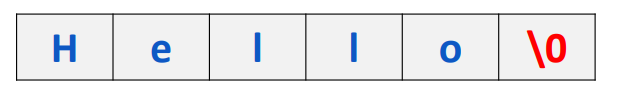
\includegraphics[width=0.8\linewidth]{img/capitolo2/hello.png}
    \label{fig:hello}
\end{figure}

Vediamo un buffer di 6 caratteri dei quali i primi 5 sono la stringa “Hello” e poi c'è il terminatore che
possiede un byte pari a zero. Questo byte è detto \textbf{NUL character} ed è diverso da NULL; infatti, per non fare
confusione lo chiameremo NIL.

Altro aspetto è l'\textbf{allocazione di un array}: per allocare un buffer in C scriviamo la classica notazione per array
e nell'esempio abbiamo 10 caratteri di cui 9 al massimo sono disponibili e uno per il terminatore. Il linguaggio
C prevede che dobbiamo creare sempre un array di dimensione almeno pari a tale dimensione, ma lo
standard non dice nulla se ne allochiamo uno di dimensione minore.

Vediamo adesso un esempio della funzione \textbf{gets()} che legge da tastiera una stringa, e di come a livello di
codice esista una vulnerabilità di tipo buffer overflow.

\begin{figure}[H]
    \centering
    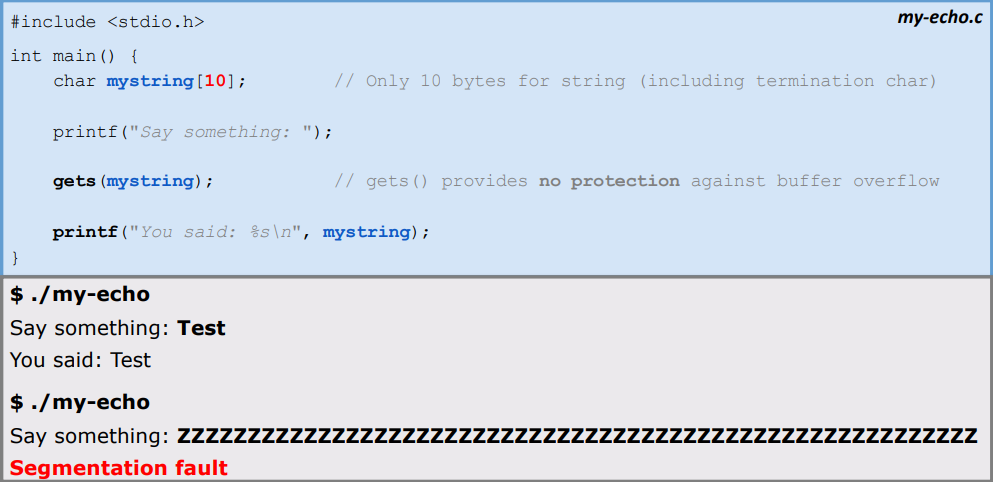
\includegraphics[width=0.9\linewidth]{img/capitolo2/gets.png}
    \label{fig:gets}
\end{figure}

Quindi se scriviamo qualcosa con meno di 9 caratteri tutto va per il meglio, se ne usiamo di più il programma
ci restituisce segmentation fault e quindi il processo viene ucciso dal SO. Questo accade perché la funzione
\textit{gets()} non fa controlli sulla dimensione dell'input e questo causa una sovrascrittura delle locazioni di memoria
contigue al buffer allocato nello stack.

\section{Mappatura della memoria dei processi}

Quando eseguiamo un programma abbiamo a disposizione una memoria virtuale (quindi byte liberi) dove
può mettere tutti i suoi dati e tutto il suo codice che è fatta in questo modo:

\begin{figure}[H]
    \centering
    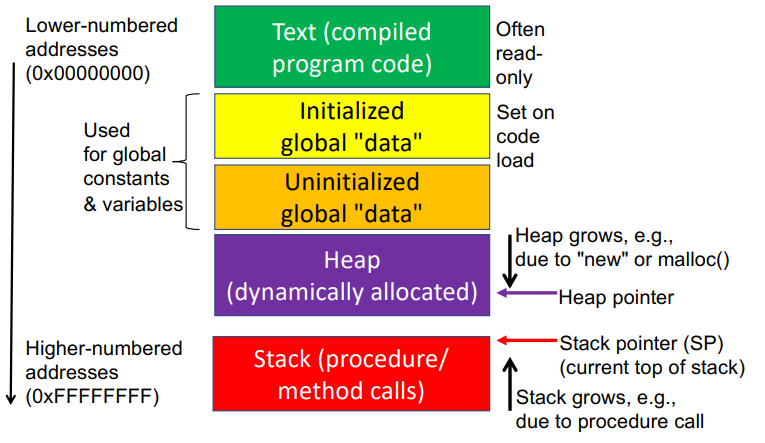
\includegraphics[width=0.8\linewidth]{img/capitolo2/stack.png}
    \label{fig:stack}
\end{figure}

L'esempio è per uno spazio di memoria composto da $2^{32}$ byte per un totale di 4 GB (\textit{0xFFFFFFFF}).

\begin{itemize}
    \item \textbf{Area testo} (in verde): corrisponde ad una copia del programma
    che lanciamo. Generalmente è accessibile in sola lettura.
    \item \textbf{Area dati globali}: tutte le variabili dichiarate fuori dal
    main o dalle funzioni. Quest'area viene ulteriormente divisa in: \textbf{Global data inizializzati}
    e \textbf{Global data non inizializzati}.
    \item \textbf{Area heap}: usata quando usiamo funzioni come malloc() o new.
    \item \textbf{Area stack}: usata per la chiamata a sottofunzione e per il 
    salvataggio delle variabili locali.
\end{itemize}

\section{Stack overflow}

Concentriamoci per ora sullo stack overflow e per tale motivo dobbiamo capire come funziona lo stack.
Lo stack viene richiamato ogni volta che chiamiamo una funzione e nello stack vengono salvati:

\begin{itemize}
    \item L'indirizzo di ritorno ("da dove vengo").
    \item I parametri di chiamata (variabili di input).
    \item Le variabili locali (se vengono create dalla funzione).
    \item Il valore di ritorno pure sullo stack.
\end{itemize}

Vediamo un esempio dove sopra abbiamo un main in C e sotto il codice assembly.

\begin{figure}[H]
    \centering
    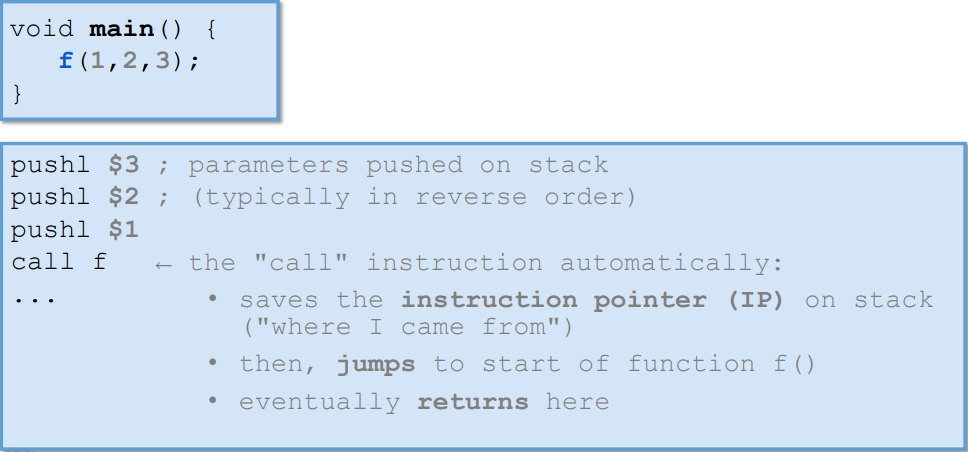
\includegraphics[width=0.8\linewidth]{img/capitolo2/call.png}
    \label{fig:call}
\end{figure}

Possiamo quindi osservare che in primo luogo si fa un push sullo stack dei parametri in input e
successivamente si chiama la funzione “\textit{f}” (f è in realtà una label a cui è associata l'indirizzo della prima
istruzione della funzione a cui saltare). In realtà se la funzione avesse avuto anche il parametro di output,
sarebbe stato pushato in memoria spazio sufficiente per tale parametro prima dei parametri di input.
Osserviamo inoltre che i parametri di input per convenzione vengono pushati in ordine inverso. Abbiamo
quindi in questa immagine quattro push, perché si conta anche \textit{call} che fa una push sullo stack.

Tipicamente \textbf{lo stack cresce dal basso verso l'alto} (quindi per indirizzi
decrescenti), SP (stack pointer) indica la cima dello stack e l'indirizzo di ritorno
viene messo sopra i tre parametri. Quindi rifacendoci all'esempio precedente
avremo sullo stack la seguente allocazione:

\begin{figure}[H]
    \centering
    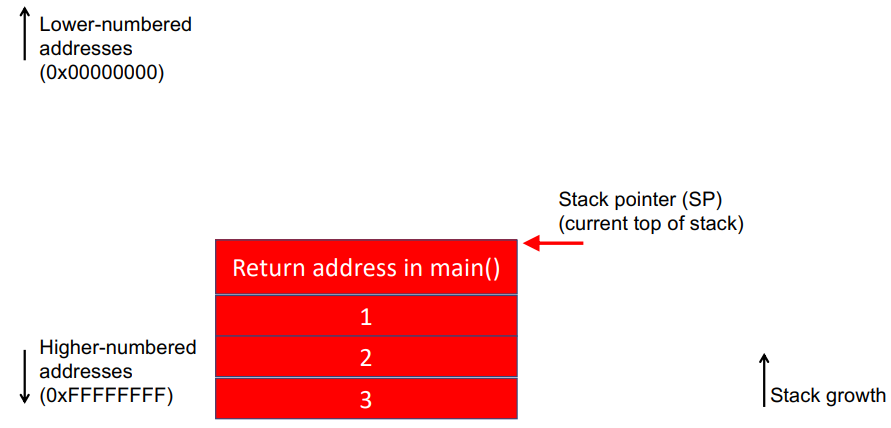
\includegraphics[width=0.8\linewidth]{img/capitolo2/stack1.png}
    \label{fig:stack1}
\end{figure}

Vediamo ora una possibile implementazione della funzione f: questa possiede 
due buffer locali, la dimensione totale del buffer richiesto sarà da 15 
byte ed infatti il codice assembly userà una \textit{subl} con un valore 
pari alla somma delle due variabili locali. Il valore \$20 è in esadecimale 
ed è pari a 32 (il compilatore alloca più spazio di quello di cui ha bisogno).

\begin{figure}[H]
    \centering
    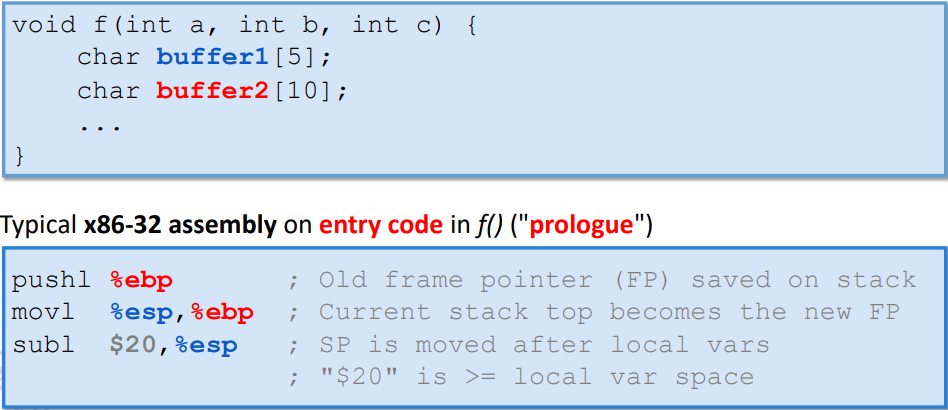
\includegraphics[width=0.8\linewidth]{img/capitolo2/function.png}
    \label{fig:function}
\end{figure}

Lo \textbf{SP} viene fatto salire sopra a tutto e vengono collocati i due buffer, ma viene prima aggiunto il valore
associato all'old frame pointer, per poi aggiornare il registro del frame pointer; ovvero il registro \%\textit{ebp}, con
il suo nuovo valore dato dallo SP. Ricordiamo infatti che il \textbf{frame pointer (FP)} è un registro in cui viene salvato
l'indirizzo associato alla prima locazione liberà dove verranno allocate le variabili locali: questo è un registro
che consente di accedere in modo semplice allo \textbf{stack frame} (ovvero alla parte dello stack dove vengono
allocate le variabili locali).

\begin{figure}[H]
    \centering
    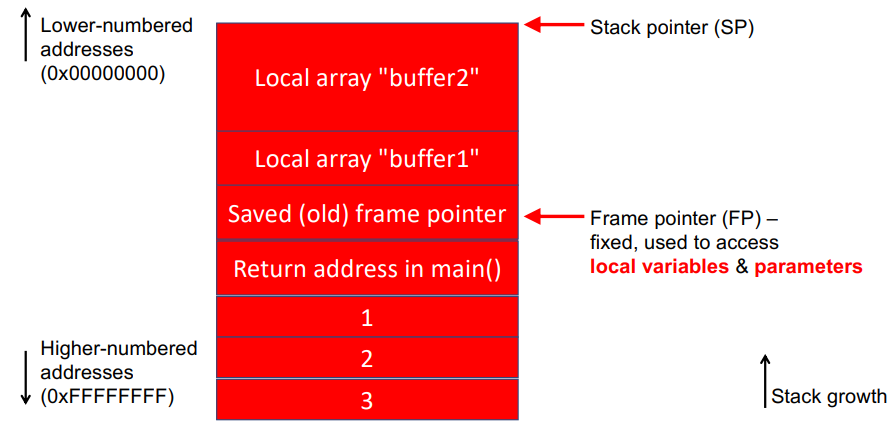
\includegraphics[width=0.8\linewidth]{img/capitolo2/stack2.png}
    \label{fig:stack2}
\end{figure}

Comprendiamo che se ad esempio usiamo \textit{gets} per inserire un valore dentro a buffer2 allora ciò che accadrà
è che avremo un buffer overflow ovvero l'input fornito sfonda il buffer e quindi partendo dall'alto scende
fino alla base dello stack. Questo vuol dire che tutti i pezzi sotto vengono sovrascritti ed il punto critico che
stiamo modificando è il return value.

Se l'input viene forgiato ad arte allora comprendiamo che è possibile iniettare del codice all'interno del buffer
e modificare il return address per far si che questo punterà al codice iniettato che chiaramente verrà
eseguito. Un possibile risultato di un attacco sarà:

\begin{figure}[H]
    \centering
    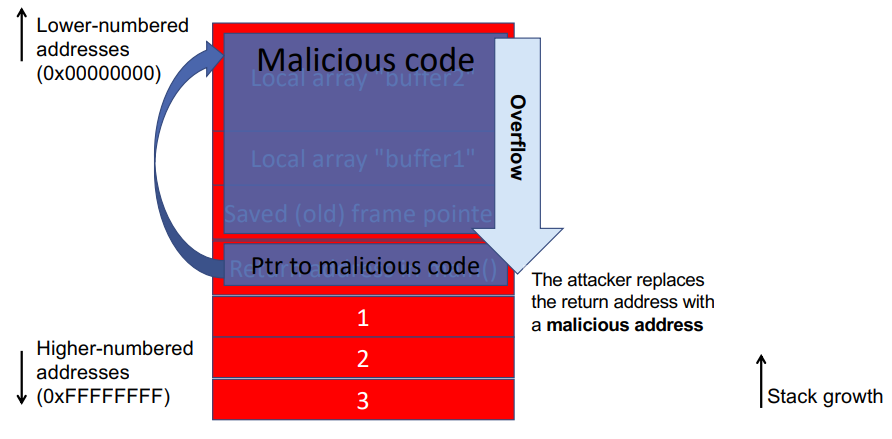
\includegraphics[width=0.8\linewidth]{img/capitolo2/stack3.png}
    \label{fig:stack3}
\end{figure}

La cosa più importante da capire oggi è: \textbf{come calcolare l'indirizzo da mettere nel return pointer}.

L'arte di creare un messaggio di buffer overflow è sartoriale per cui un pezzo di codice finisce nel mezzo dello
stack, alla fine invece abbiamo un indirizzo e il \textbf{NOP Sled} (che è un riempitivo).

\begin{figure}[H]
    \centering
    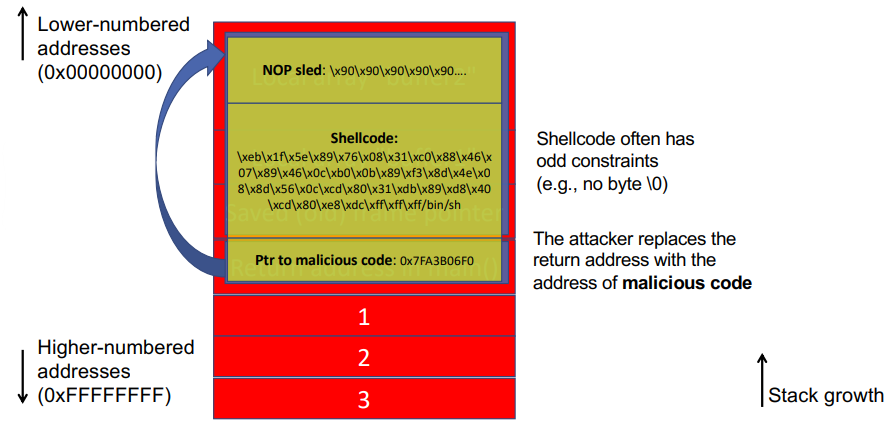
\includegraphics[width=0.8\linewidth]{img/capitolo2/stack4.png}
    \label{fig:stack4}
\end{figure}

\section{Prevenzione buffer overflow}

La cosa più naturale e semplice è quella di scartare tutte le funzioni che non sono sicure by-design, quindi:

\begin{itemize}
    \item \textit{gets()}, legge l'input senza controllarlo
    \item \textit{strcpy()}, \textit{strcat()}, copia e concatenazione da sorgente a destinazione e non hanno un limite
    \item altre funzioni possono essere: \textit{scanf()}, \textit{fscanf()}, \textit{sscanf()} e tante altre
    \item non solo funzioni, anche dei semplici cicli possono causare overflow
\end{itemize}

Quelle che \textbf{apparentemente sembrano sicure} sono: \textit{strncpy()}, \textit{strncat}, \textit{snprintf}.
Ma perché sono apparentemente sicure? Prima di tutto perché non sono di facile utilizzo, in secondo
presentano alcuni problemi. Ad esempio, la funzione di copia o concatenamento non usa il terminatore.

\section{Contromisure buffer overflow}

Esistono due macro-famiglie di difese:

\begin{itemize}
    \item Approcci basati su Compilatori
    \begin{itemize}
        \item Canarino
        \item LibSafe
        \item Alternative inserite dal compilatore
    \end{itemize}
    \item Approcci basati a tempo di esecuzione/SO
    \begin{itemize}
        \item Stack non eseguibile
        \item Allocazione dei dati/codice randomizzata all'interno della memoria (ASLR)
    \end{itemize}
\end{itemize}

Vediamo l'approccio basato su \textbf{canarino}. Lo stack, prima di eseguire 
la funzione immette un stringa randomica tra l'indirizzo di ritorno e il 
resto dello stack (ovvero il canarino) e questo stesso valore viene salvato 
in un registro segreto casuale e non è scritto nel programma. Supponiamo 
che vi sia stato un buffer overflow; prima di effettuare il return la
funzione legge il canarino e confronta il valore con il registro: se il 
valore non coincide allora c'è stato un problema e viene bloccata 
l'esecuzione.

\begin{figure}[H]
    \centering
    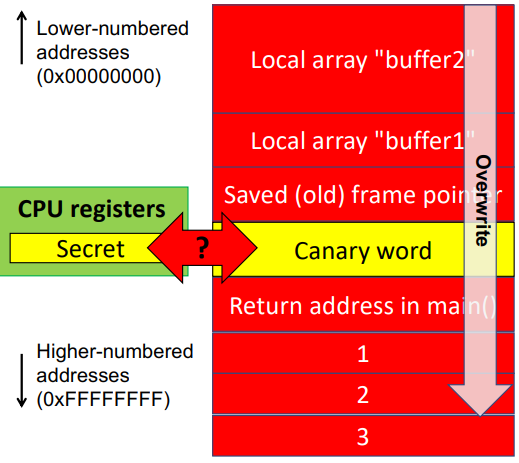
\includegraphics[width=0.5\linewidth]{img/capitolo2/stack5.png}
    \label{fig:stack5}
\end{figure}

Vi è poi un altro elenco di difese e attacchi, ma spesso sembra giocare al gatto e al topo:

\begin{enumerate}
    \item Se la difesa è non rendere eseguibile lo stack/heap ciò che si fa è piuttosto che iniettare lo shell code,
    chiamiamo una funzione di libreria e quindi una primitiva.
    \item Se la difesa è nascondere l'indirizzo delle funzioni di libreria (libc code) o si adottano tecniche ASLR
    si possono provare attacchi a forza bruta il cui compito è individuare tale indirizzo.
    \item Se la difesa è non usare il codice della libc abbiamo come possibile attacco la costruzione delle
funzioni di cui si ha bisogno sfruttando il return oriented programming (ROP).
\end{enumerate}

Anche se esistono difese non è detto che queste vengono adottate; ad esempio molti prodotti IoT non lo
fanno.
